\chapter{Marco de referencia}

\section{Antecedentes}

La empresa Bypasa S.A. de C.V. diseña y fabrica componentes antivibratorios para el sector 
automovilístico, partiendo desde la creación de los materiales poliméricos requeridos, la 
selección de la geometría y la validación del diseño. Sin embargo los herramentales: moldes y troqueles,  
que utiliza en sus procesos de producción son diseñados y fabricados por empresas extranjeras y/o 
nacionales. Por esto se está desarrollando un proyecto cuyo objetivo es poner en operación un centro 
de diseño, fabricación y validación de moldes y troqueles.\\

El modelado y simulación, por medio de métodos numéricos computacionales, de los procesos de fabricación 
involucrados en el desarrollo de los herramentales es una parte importante del proyecto, puesto que 
permitirá tomar decisiones respecto a los diseños en etapas tempranas, minimizando los costos derivados de 
los ajustes realizados después de ejecutar corridas de prueba.

\section{Planteamiento del problema}

Se requiere simular el proceso de formado de un tubo de acero SAE 1018 que será fabricado con el herramental 
diseñado en el nuevo centro de desarrollo. 

\section{Estado del arte}

La posibilidad de desarrollar simulaciones de los procesos de estampados metálicos fue durante mucho tiempo 
un deseo inalcanzable para la industria de estampados. Los ingenieros de procesos esperaban ser capaces de 
identificar posibles defectos en el formado en etapas tempranas de diseño y/o desarrollo de los herramentales, 
y minimizar la necesidad de modificaciones costosas de las herramientas en una serie de procesos de ensayo y error. \\

El modelado de problemas de estampado de partes metálicas requiere una precisión considerable en la caracterización 
de efectos como el comportamiento no lineal de un material, grandes deformaciones y condiciones de contacto entre la
herramienta y la parte a estampar.que derivan  en algoritmos complejos.~\cite{banabic2000}\\

La primera formulación teóricamente correcta de problemas de formado de metales fue presentada por Wang y Budiansky 
~\cite{wang1978} en 1978. El método presentado fue una formulación total lagrangiana e involucraba elementos triangulares membrana de 
deformación constante. La solución implementada fue un esquema incremental Euleriano hacia adelante. Los métodos basados en un 
esquema de solución como el anterior son llamados como métodos estáticos-explícitos.\\

En el inicio de la década de los 90's hubo un incremento considerable en la utilización de la simulación de estampado 
metálico dentro de la industria y a mediados de esta década la mayoría de las compañías en la industria automotriz 
establecieron las simulaciones de estampado como aspectos elementales en el desarrollo de sus procesos. 
Actualmente existen programas de computadora altamente especializados en la simulación de estampados, siendo AutoForm 
uno de los más utilizados, este surgió como un proyecto de investigación en el ETH de Zurich en los inicios de los 90's. 
El código está basado en un enfoque estático-implícito, pero utiliza algunos algoritmos innovativos que le permiten 
una estabilidad y eficiencia computacional competitiva respecto a los códigos de tipo dinámico-explícito.~\cite{banabic2000}

Huang & Leu ~\cite{huang1995} desarrollaron un código de análisis elasto-plástico por elemento finito, basado en una formulación 
lagrangiana modificada, para simular proceso de doblado UO en placas metálicas, bajo condiciones de deformación 
plana. Para realizar el análisis del proceso completo, dividieron este en tres pasos de carga o configuraciones 
que se muestran en la figura 1, doblado en U, descarga y doblado final en O. Aplicaron además simetría debido a la 
disposicion de las herramientas y el blank a formar, simplificando aún más el análisis. Utilizaron un coeficiente 
de fricción de $\mu = 0.02$ y el espesor de la chapa fue de 6 mm.\\

En la figura 2 se puede observar la secuencia del desarrollo de la geometría obtenida mediante el análisis 
realizado. 

\begin{center}
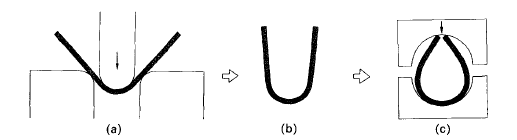
\includegraphics[scale=0.95]{src/uo-bending.png}
\captionof{figure}{Proceso de doblado UO, a) Doblado en U b) Descarga c) Doblado en O \textit{Fuente: Huang (1995)}}
\end{center}

\begin{center}
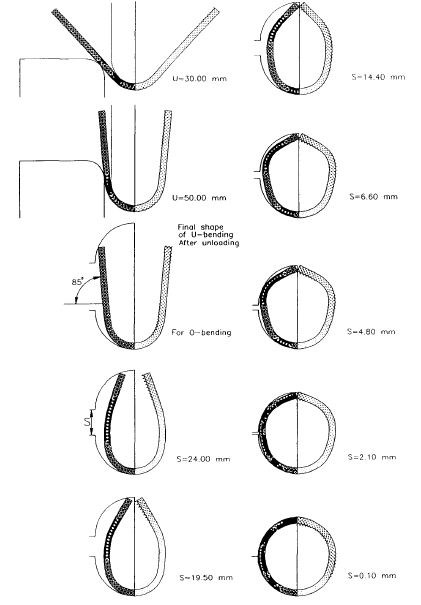
\includegraphics[scale=0.8]{src/shape_sequence.png}
\captionof{figure}{Secuencia obtenida mediante el proceso de doblado UO. \textit{Fuente: Huang (1995)}}
\end{center}


\section{Justificación}

La simulación por elemento finito en el proceso de diseño de herramentales, así como en 
la simulación de procesos de estampado es una herramienta muy útil, puesto que representa un ahorro 
significativo de costos y tiempo, a la vez que permite establecer una metodología de trabajo más efectiva, minimizando las 
actividades de tipo prueba-error para la realización de ajustes.\\

Además de lo anterior, la simulación presenta la ventaja de poder variar parámetros que influyen en los procesos de 
estampado, de manera conveniente, sin que esto derive en gastos excesivos de recursos, con la finalidad de entender 
de mejor manera la influencia de ciertas propiedades o condiciones, e inclusive optimizar las características 
de un componente.

% \section{Hipótesis}

% Es posible simular el desarrollo del formado de un tubo para buje utilizando un software de simulación 
% por elemento finito y utilizar estos resultados como una herramienta auxiliar en el desarrollo de 
% nuevos herramentales.

\section{Objetivo general}

Simular y validar el proceso de formado de un tubo de acero SAE 1018.

\section{Objetivos particulares}
\begin{itemize}
\item Simular el desarrollo de formado del tubo.
\item Identificar fallas potenciales o características no deseables en el tubo.
\item Calcular de la fuerza requerida para completar el proceso de formado.
\item Verificar las características geométricas y dimensionales del tubo.
\item Validar los resultados de la simulación.
%\item Caracterizar de forma experimental y por elemento finito el comportamiento elástico de la materia prima utilizada.
\end{itemize}


\section{Alcances}
\begin{itemize}
\item Desarrollo de un modelo de elemento finito del proceso de formado de un tubo.
\item Publicación de un artículo.
\end{itemize}

